\subsection{Population Generation}

% Short description
The PopulationGenerator function produces an intensity map representing the population density across the terrain (see Table \ref{table:popgen}).
The terrain parameter is required since certain areas of the terrain need to be masked off from population, such as oceans, rivers, and spiky mountain tops.
\begin{table}[H]
  \centering
  \begin{tabular}{lllll}
    \textbf{Input}                           &               & \textbf{Function}            &               & \textbf{Output}         \\
    \midrule
    \textit{Terrain, PopulationAmplifier[]}      & $\rightarrow$ & \textbf{PopulationGenerator}      & $\rightarrow$ & \textit{PopulationMap}        \\
    \bottomrule
  \end{tabular}

  \caption{Definition of the PopulationGenerator function which is responsible for generating an intensity map of population across the terrain.}
  \label{table:popgen}
\end{table}
\vspace{-0.4cm} % Mimic spacing below figures

The other input parameter is a set of amplifiers.
Each amplifier is a 2D geometry visually represented with markers that give covered areas drastically increased population.
Through these amplifiers, the user may designate locations of city centers, and thus interactively modify the population across the terrain.
An example of this usage can be found in Figure \ref{fig:pop_dens}.

To generate the initial population distribution, the generator was implemented with a few layers of simplex noise.
The population amplifiers from the function input are applied after this initial population map has been generated.
The noise logic was eventually extracted into a separate module, which was then shared with the terrain generator, although with different manually designed layers.

\begin{figure}[h!]
  \centering
  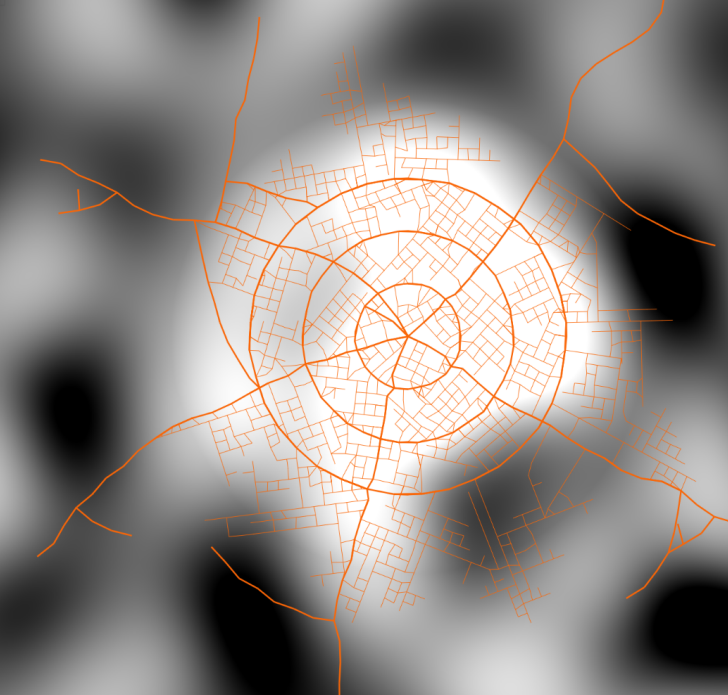
\includegraphics[width=0.35\textwidth]{figure/pop_density.png}
  \caption{An example of a population map with a Paris city generated within it.}
  \label{fig:pop_dens}
\end{figure}